\chapter{Configuring Hbase in Standalone & Pseudo-distributed mode}
%Intro\footnotemark\\
\par Lorem ipsum dolor sit amet, consectetur adipiscing elit. Aliquam facilisis massa quis orci volutpat, ut dictum tellus pulvinar. Nam vulputate diam a leo dignissim varius. Aenean nec tellus malesuada, tristique libero vitae, lacinia nibh. Donec quam libero, accumsan sollicitudin massa a, dictum gravida mauris.
\begin{spacing}{1.2}
%note en bas de page
\section{Preparating environment }
\par Lorem ipsum dolor sit amet, consectetur adipiscing elit. Aliquam facilisis massa quis orci volutpat, ut dictum tellus pulvinar. Nam vulputate diam a leo dignissim varius. Aenean nec tellus malesuada, tristique libero vitae, lacinia nibh. Donec quam libero, accumsan sollicitudin massa a, dictum gravida mauris
\\
\begin{figure}[!htb] 
\begin{center} 
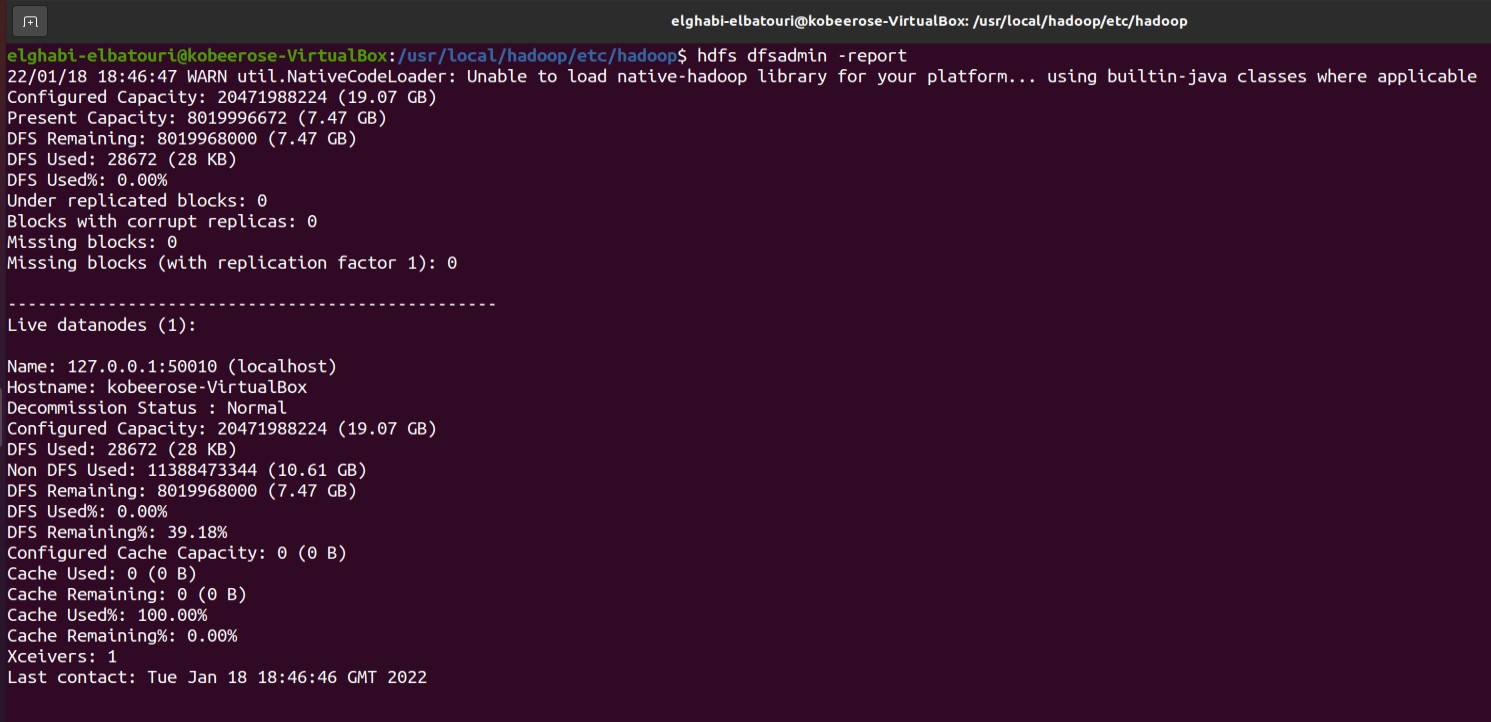
\includegraphics[width=1\linewidth]{Pictures/HBase/Configuring Hbase in Standalone & Pseudo-distributed mode/Preparating environment/hdfs report} 
\end{center} 
\caption{hdfs report} 
\end{figure}  \FloatBarrier
\\
\section{Installing and Configuring Apache Hbase }
\par Lorem ipsum dolor sit amet, consectetur adipiscing elit. Aliquam facilisis massa quis orci volutpat, ut dictum tellus pulvinar. Nam vulputate diam a leo dignissim varius. Aenean nec tellus malesuada, tristique libero vitae, lacinia nibh. Donec quam libero, accumsan sollicitudin massa a, dictum gravida mauris
\\
\begin{figure}[!htb] 
\begin{center} 
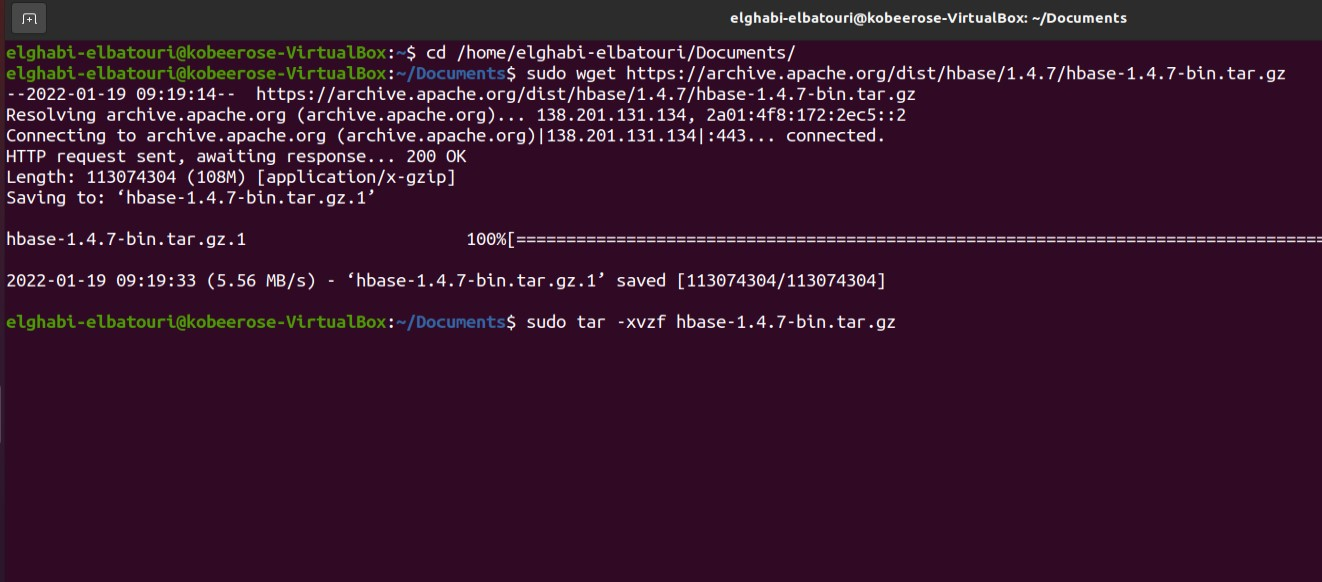
\includegraphics[width=1\linewidth]{Pictures/HBase/Configuring Hbase in Standalone & Pseudo-distributed mode/Installing and Configuring Apache Hbase/Download Hbase} 
\end{center} 
\caption{Download Hbase} 
\end{figure}  \FloatBarrier
\\

\par Lorem ipsum dolor sit amet, consectetur adipiscing elit. Aliquam facilisis massa quis orci volutpat, ut dictum tellus pulvinar. Nam vulputate diam a leo dignissim varius. Aenean nec tellus malesuada, tristique libero vitae, lacinia nibh. Donec quam libero, accumsan sollicitudin massa a, dictum gravida mauris
\\
\begin{figure}[!htb] 
\begin{center} 
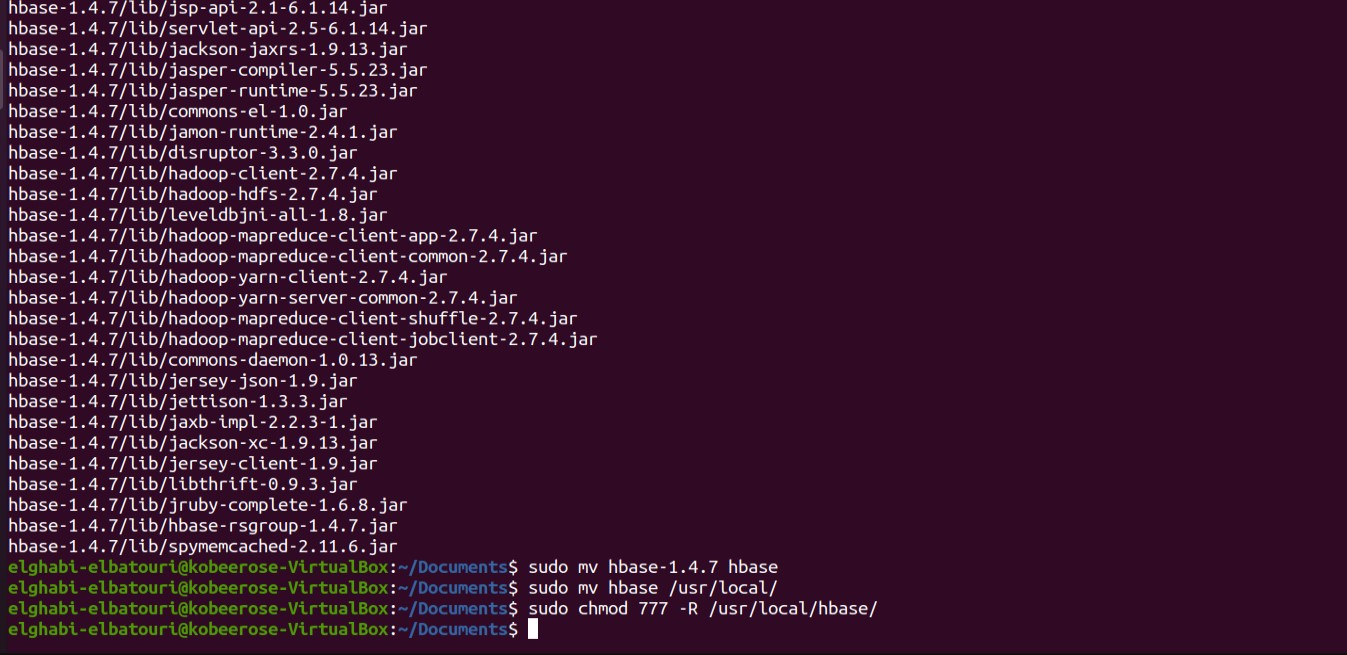
\includegraphics[width=1\linewidth]{Pictures/HBase/Configuring Hbase in Standalone & Pseudo-distributed mode/Installing and Configuring Apache Hbase/Extracting and moving Hbase folder} 
\end{center} 
\caption{Extracting and moving Hbase folder} 
\end{figure}  \FloatBarrier
\\

\par Lorem ipsum dolor sit amet, consectetur adipiscing elit. Aliquam facilisis massa quis orci volutpat, ut dictum tellus pulvinar. Nam vulputate diam a leo dignissim varius. Aenean nec tellus malesuada, tristique libero vitae, lacinia nibh. Donec quam libero, accumsan sollicitudin massa a, dictum gravida mauris
\\
\begin{figure}[!htb] 
\begin{center} 
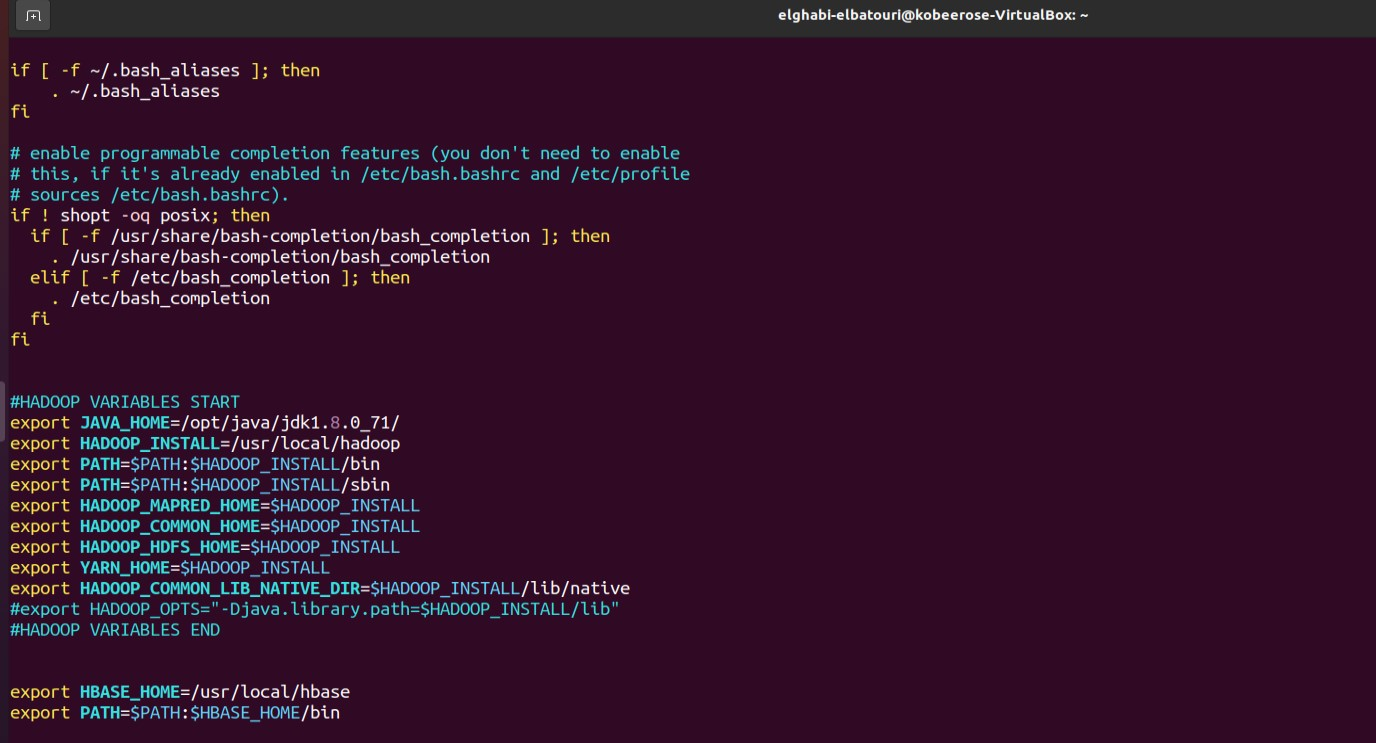
\includegraphics[width=1\linewidth]{Pictures/HBase/Configuring Hbase in Standalone & Pseudo-distributed mode/Installing and Configuring Apache Hbase/Adding Hbase path to .bashrc} 
\end{center} 
\caption{Adding Hbase path to .bashrc} 
\end{figure}  \FloatBarrier
\\

\par Lorem ipsum dolor sit amet, consectetur adipiscing elit. Aliquam facilisis massa quis orci volutpat, ut dictum tellus pulvinar. Nam vulputate diam a leo dignissim varius. Aenean nec tellus malesuada, tristique libero vitae, lacinia nibh. Donec quam libero, accumsan sollicitudin massa a, dictum gravida mauris
\\
\begin{figure}[!htb] 
\begin{center} 
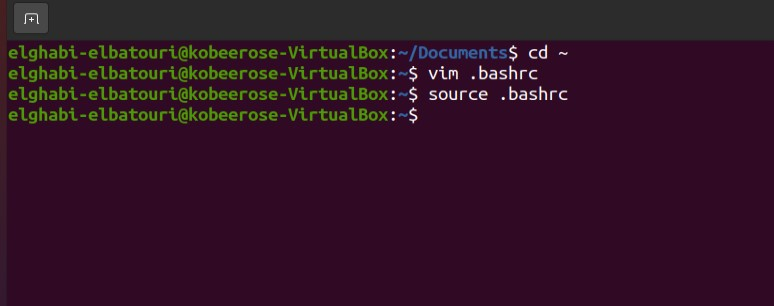
\includegraphics[width=1\linewidth]{Pictures/HBase/Configuring Hbase in Standalone & Pseudo-distributed mode/Installing and Configuring Apache Hbase/Update current shell environment} 
\end{center} 
\caption{Update current shell environment} 
\end{figure}  \FloatBarrier
\\

\par Lorem ipsum dolor sit amet, consectetur adipiscing elit. Aliquam facilisis massa quis orci volutpat, ut dictum tellus pulvinar. Nam vulputate diam a leo dignissim varius. Aenean nec tellus malesuada, tristique libero vitae, lacinia nibh. Donec quam libero, accumsan sollicitudin massa a, dictum gravida mauris
\\
\begin{figure}[!htb] 
\begin{center} 
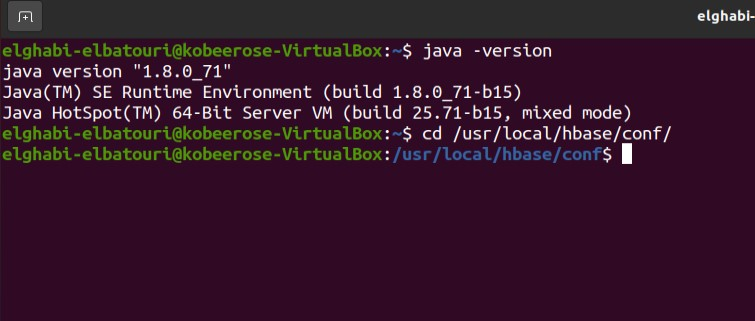
\includegraphics[width=1\linewidth]{Pictures/HBase/Configuring Hbase in Standalone & Pseudo-distributed mode/Installing and Configuring Apache Hbase/Checking Java version} 
\end{center} 
\caption{Checking Java version} 
\end{figure}  \FloatBarrier
\\

\par Lorem ipsum dolor sit amet, consectetur adipiscing elit. Aliquam facilisis massa quis orci volutpat, ut dictum tellus pulvinar. Nam vulputate diam a leo dignissim varius. Aenean nec tellus malesuada, tristique libero vitae, lacinia nibh. Donec quam libero, accumsan sollicitudin massa a, dictum gravida mauris
\\
\begin{figure}[!htb] 
\begin{center} 
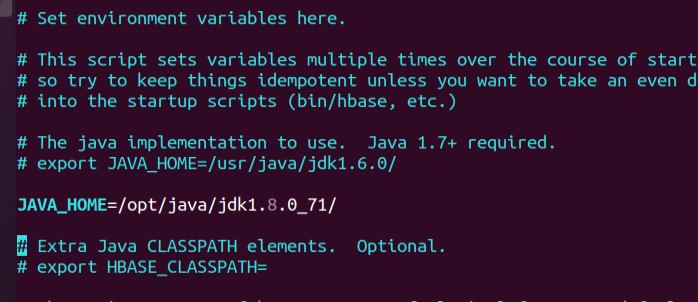
\includegraphics[width=1\linewidth]{Pictures/HBase/Configuring Hbase in Standalone & Pseudo-distributed mode/Installing and Configuring Apache Hbase/Adding JAVA_HOME to hbase-env.sh file} 
\end{center} 
\caption{Adding JAVA_HOME to hbase-env.sh file} 
\end{figure}  \FloatBarrier
\\

\par Lorem ipsum dolor sit amet, consectetur adipiscing elit. Aliquam facilisis massa quis orci volutpat, ut dictum tellus pulvinar. Nam vulputate diam a leo dignissim varius. Aenean nec tellus malesuada, tristique libero vitae, lacinia nibh. Donec quam libero, accumsan sollicitudin massa a, dictum gravida mauris
\\
\begin{figure}[!htb] 
\begin{center} 
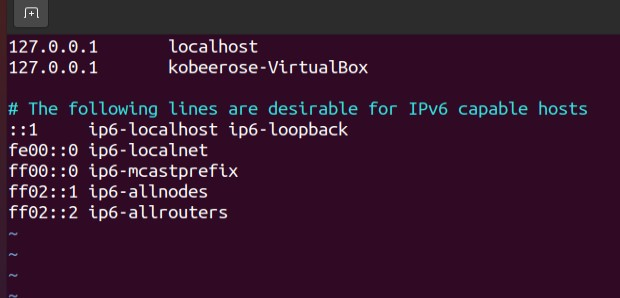
\includegraphics[width=1\linewidth]{Pictures/HBase/Configuring Hbase in Standalone & Pseudo-distributed mode/Installing and Configuring Apache Hbase/Changing IP adresse of host} 
\end{center} 
\caption{Changing IP adresse of host} 
\end{figure}  \FloatBarrier
\\

\par Lorem ipsum dolor sit amet, consectetur adipiscing elit. Aliquam facilisis massa quis orci volutpat, ut dictum tellus pulvinar. Nam vulputate diam a leo dignissim varius. Aenean nec tellus malesuada, tristique libero vitae, lacinia nibh. Donec quam libero, accumsan sollicitudin massa a, dictum gravida mauris
\\
\begin{figure}[!htb] 
\begin{center} 
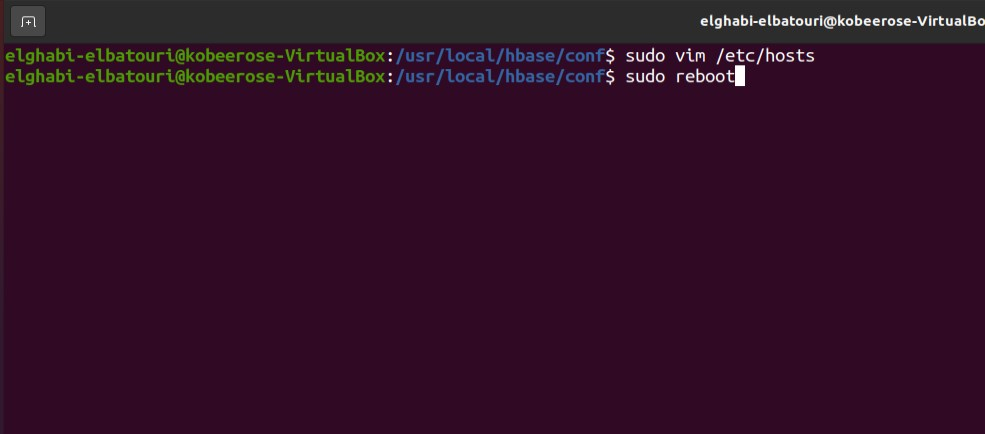
\includegraphics[width=1\linewidth]{Pictures/HBase/Configuring Hbase in Standalone & Pseudo-distributed mode/Installing and Configuring Apache Hbase/rebooting the machine} 
\end{center} 
\caption{rebooting the machine} 
\end{figure}  \FloatBarrier
\\

\par Lorem ipsum dolor sit amet, consectetur adipiscing elit. Aliquam facilisis massa quis orci volutpat, ut dictum tellus pulvinar. Nam vulputate diam a leo dignissim varius. Aenean nec tellus malesuada, tristique libero vitae, lacinia nibh. Donec quam libero, accumsan sollicitudin massa a, dictum gravida mauris
\\
\begin{figure}[!htb] 
\begin{center} 
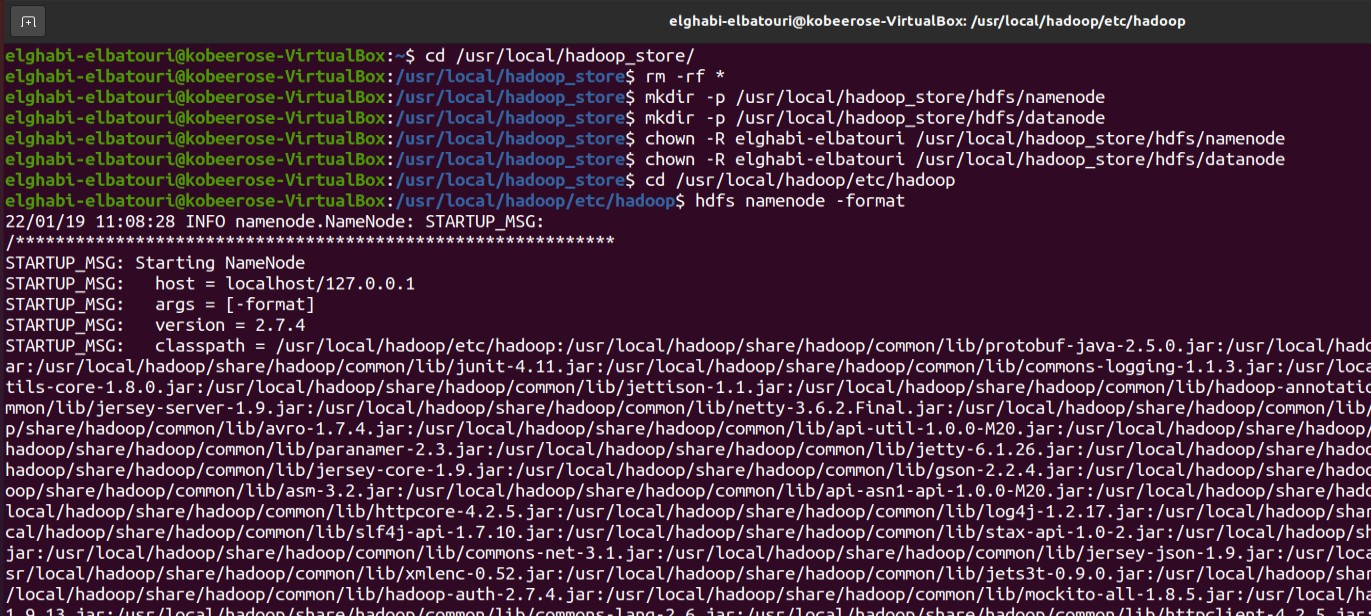
\includegraphics[width=1\linewidth]{Pictures/HBase/Configuring Hbase in Standalone & Pseudo-distributed mode/Installing and Configuring Apache Hbase/Cleaning the hadoop_store} 
\end{center} 
\caption{Cleaning the hadoop_store} 
\end{figure}  \FloatBarrier
\\

\par Lorem ipsum dolor sit amet, consectetur adipiscing elit. Aliquam facilisis massa quis orci volutpat, ut dictum tellus pulvinar. Nam vulputate diam a leo dignissim varius. Aenean nec tellus malesuada, tristique libero vitae, lacinia nibh. Donec quam libero, accumsan sollicitudin massa a, dictum gravida mauris
\\
\begin{figure}[!htb] 
\begin{center} 
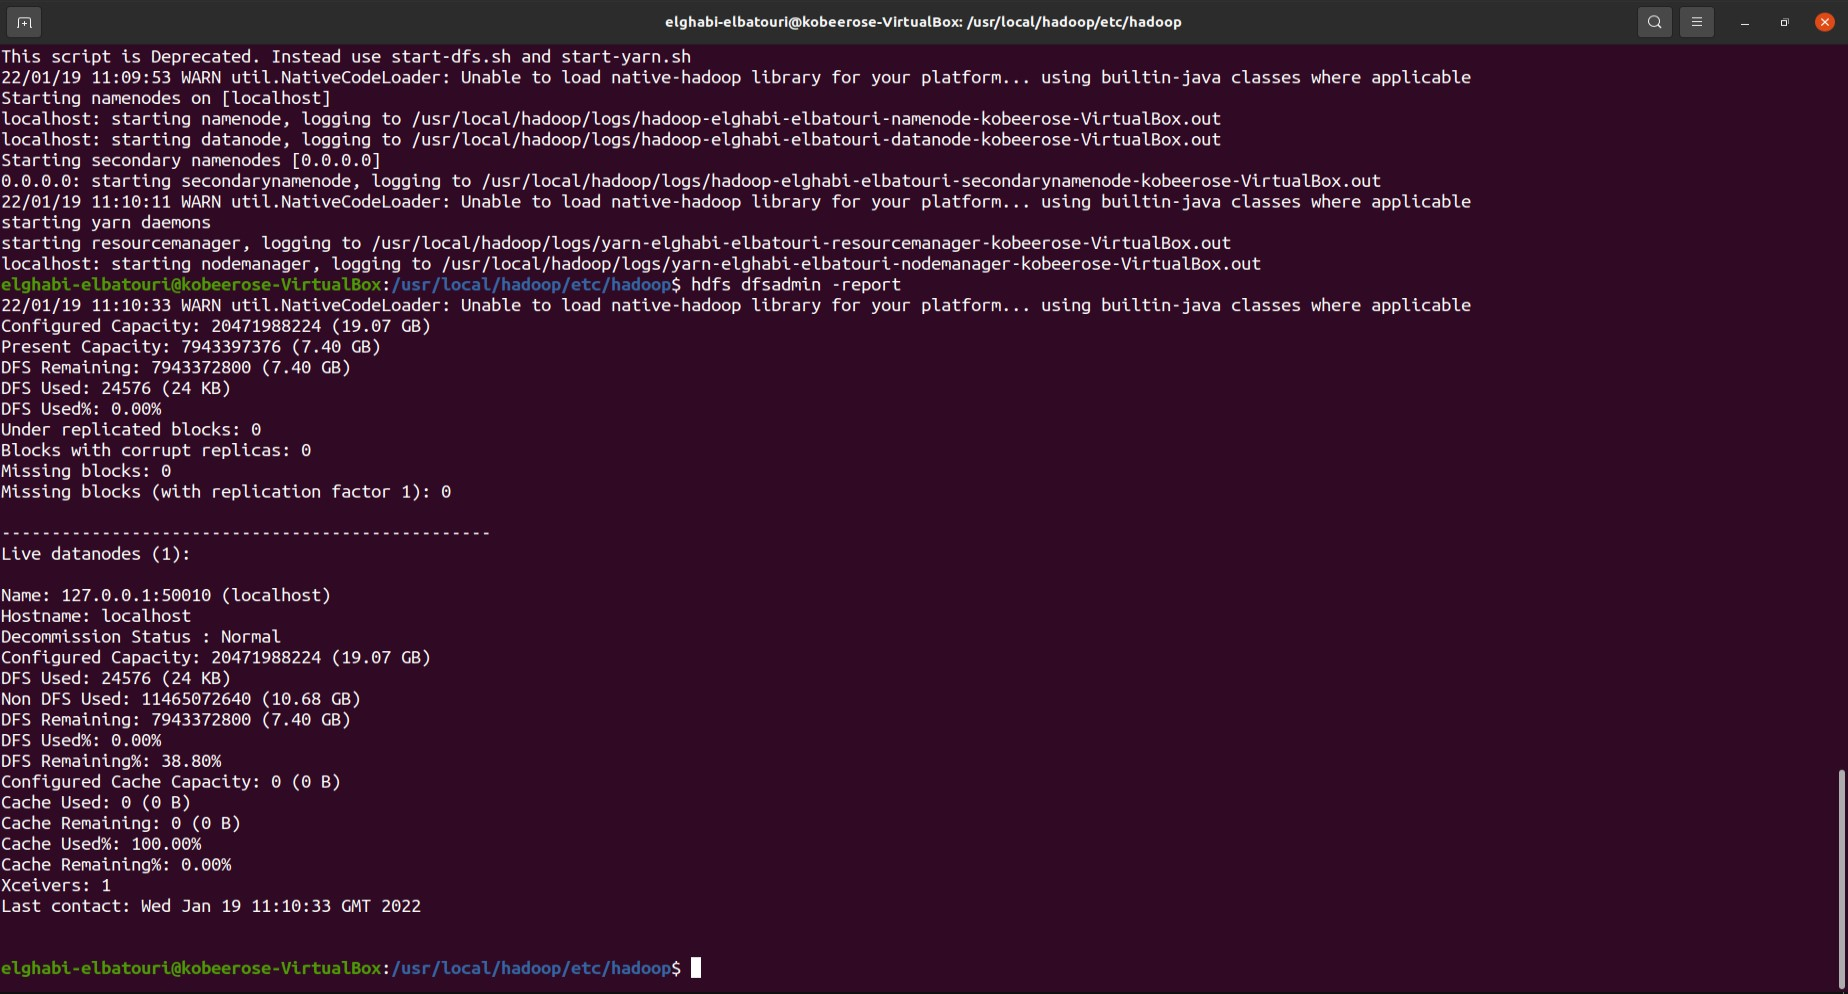
\includegraphics[width=1\linewidth]{Pictures/HBase/Configuring Hbase in Standalone & Pseudo-distributed mode/Installing and Configuring Apache Hbase/Starting hadoop daemons} 
\end{center} 
\caption{Starting hadoop daemons} 
\end{figure}  \FloatBarrier
\\
\section{Configuring Hbase in Standalone mode }
\par Lorem ipsum dolor sit amet, consectetur adipiscing elit. Aliquam facilisis massa quis orci volutpat, ut dictum tellus pulvinar. Nam vulputate diam a leo dignissim varius. Aenean nec tellus malesuada, tristique libero vitae, lacinia nibh. Donec quam libero, accumsan sollicitudin massa a, dictum gravida mauris
\\
\begin{figure}[!htb] 
\begin{center} 
\includegraphics[width=1\linewidth]{Pictures/HBase/Configuring Hbase in Standalone & Pseudo-distributed mode/Configuring Hbase in Standalone mode/Configuration of hbase-site.xml file } 
\end{center} 
\caption{Configuration of hbase-site.xml file } 
\end{figure}  \FloatBarrier
\\

\par Lorem ipsum dolor sit amet, consectetur adipiscing elit. Aliquam facilisis massa quis orci volutpat, ut dictum tellus pulvinar. Nam vulputate diam a leo dignissim varius. Aenean nec tellus malesuada, tristique libero vitae, lacinia nibh. Donec quam libero, accumsan sollicitudin massa a, dictum gravida mauris
\\
\begin{figure}[!htb] 
\begin{center} 
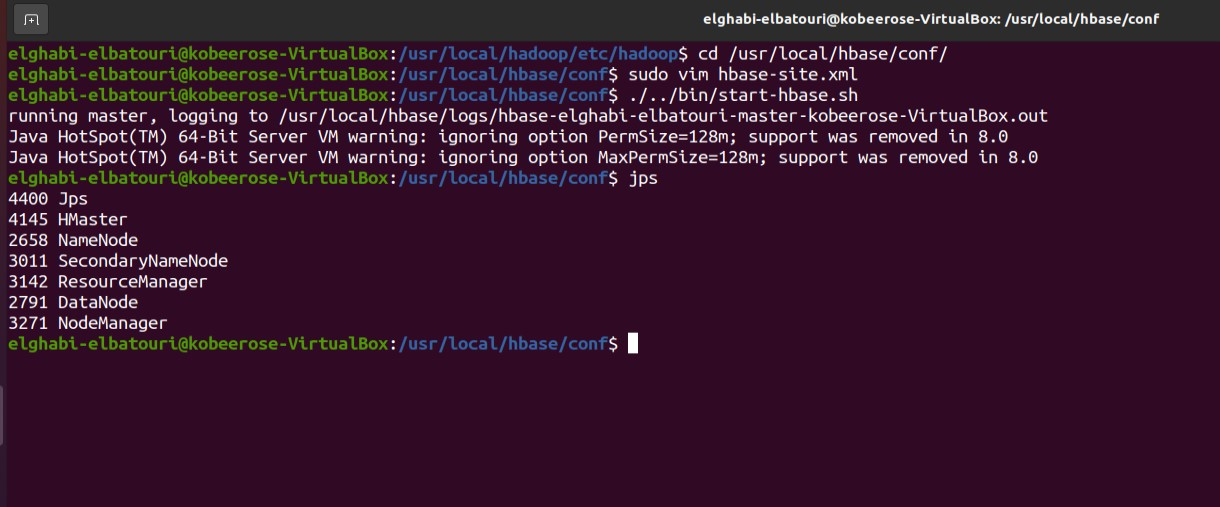
\includegraphics[width=1\linewidth]{Pictures/HBase/Configuring Hbase in Standalone & Pseudo-distributed mode/Configuring Hbase in Standalone mode/HMaster in jps} 
\end{center} 
\caption{HMaster in jps} 
\end{figure}  \FloatBarrier
\\

\par Lorem ipsum dolor sit amet, consectetur adipiscing elit. Aliquam facilisis massa quis orci volutpat, ut dictum tellus pulvinar. Nam vulputate diam a leo dignissim varius. Aenean nec tellus malesuada, tristique libero vitae, lacinia nibh. Donec quam libero, accumsan sollicitudin massa a, dictum gravida mauris
\\
\begin{figure}[!htb] 
\begin{center} 
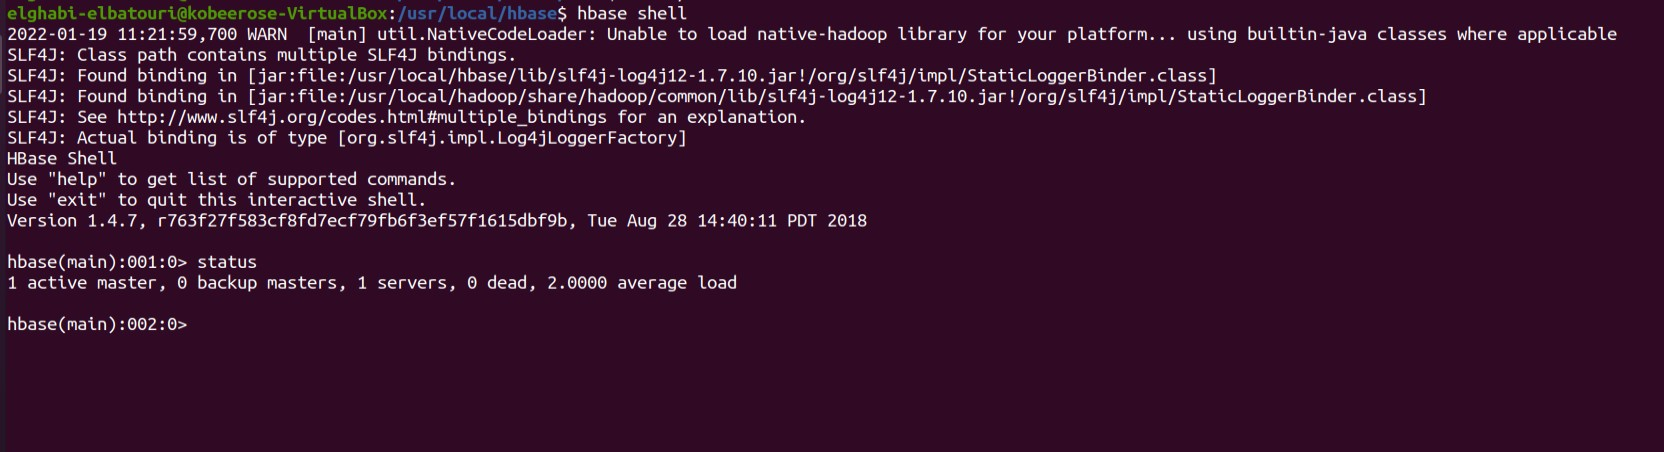
\includegraphics[width=1\linewidth]{Pictures/HBase/Configuring Hbase in Standalone & Pseudo-distributed mode/Configuring Hbase in Standalone mode/Hbase shell} 
\end{center} 
\caption{Hbase shell} 
\end{figure}  \FloatBarrier
\\

\par Lorem ipsum dolor sit amet, consectetur adipiscing elit. Aliquam facilisis massa quis orci volutpat, ut dictum tellus pulvinar. Nam vulputate diam a leo dignissim varius. Aenean nec tellus malesuada, tristique libero vitae, lacinia nibh. Donec quam libero, accumsan sollicitudin massa a, dictum gravida mauris
\\
\begin{figure}[!htb] 
\begin{center} 
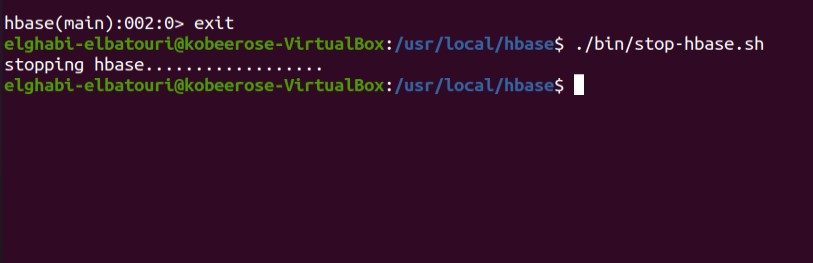
\includegraphics[width=1\linewidth]{Pictures/HBase/Configuring Hbase in Standalone & Pseudo-distributed mode/Configuring Hbase in Standalone mode/Stopping Hbase daemons} 
\end{center} 
\caption{Stopping Hbase daemons} 
\end{figure}  \FloatBarrier
\\

\par Lorem ipsum dolor sit amet, consectetur adipiscing elit. Aliquam facilisis massa quis orci volutpat, ut dictum tellus pulvinar. Nam vulputate diam a leo dignissim varius. Aenean nec tellus malesuada, tristique libero vitae, lacinia nibh. Donec quam libero, accumsan sollicitudin massa a, dictum gravida mauris
\\
\begin{figure}[!htb] 
\begin{center} 
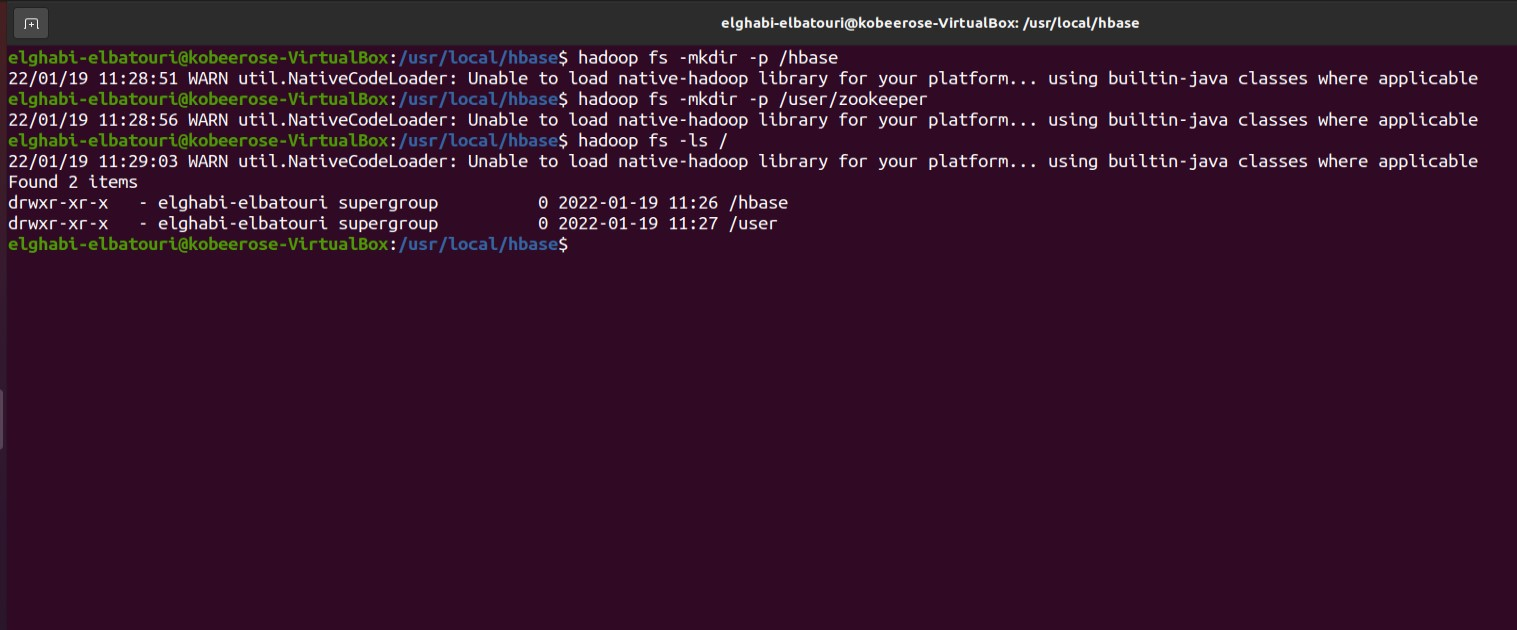
\includegraphics[width=1\linewidth]{Pictures/HBase/Configuring Hbase in Standalone & Pseudo-distributed mode/Configuring Hbase in Standalone mode/Creating Hbase repositories in Hadoop} 
\end{center} 
\caption{Creating Hbase repositories in Hadoop} 
\end{figure}  \FloatBarrier
\\
\section{Configuring Hbase in Pseudo-distributed mode }
\par Lorem ipsum dolor sit amet, consectetur adipiscing elit. Aliquam facilisis massa quis orci volutpat, ut dictum tellus pulvinar. Nam vulputate diam a leo dignissim varius. Aenean nec tellus malesuada, tristique libero vitae, lacinia nibh. Donec quam libero, accumsan sollicitudin massa a, dictum gravida mauris
\\
\begin{figure}[!htb] 
\begin{center} 
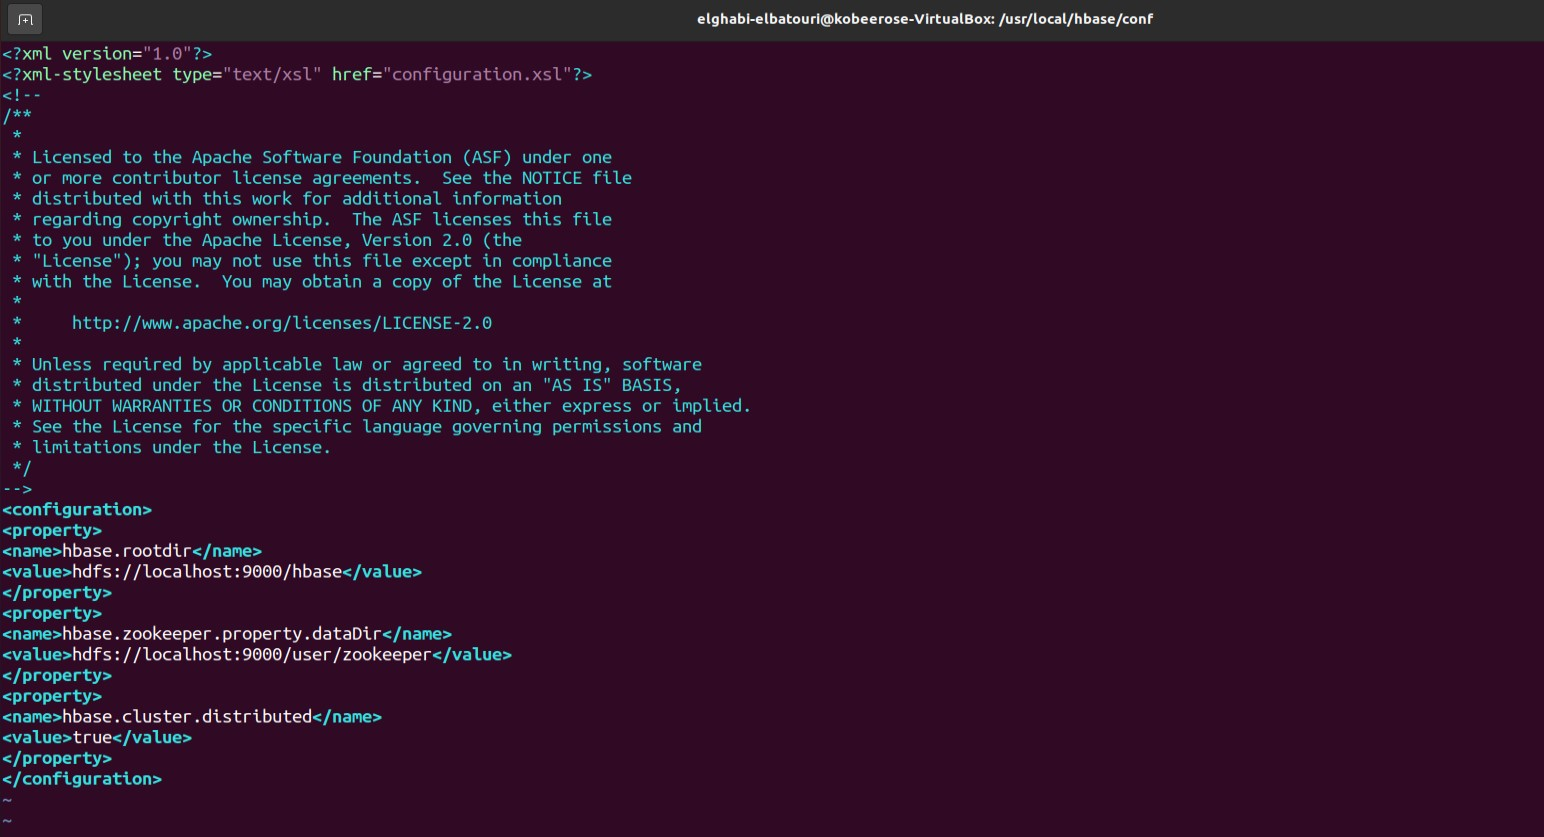
\includegraphics[width=1\linewidth]{Pictures/HBase/Configuring Hbase in Standalone & Pseudo-distributed mode/Configuring Hbase in Pseudo-distributed mode/Configuring hbase-site.xml for Distributed mode} 
\end{center} 
\caption{Configuring hbase-site.xml for Distributed mode} 
\end{figure}  \FloatBarrier
\\

\par Lorem ipsum dolor sit amet, consectetur adipiscing elit. Aliquam facilisis massa quis orci volutpat, ut dictum tellus pulvinar. Nam vulputate diam a leo dignissim varius. Aenean nec tellus malesuada, tristique libero vitae, lacinia nibh. Donec quam libero, accumsan sollicitudin massa a, dictum gravida mauris
\\
\begin{figure}[!htb] 
\begin{center} 
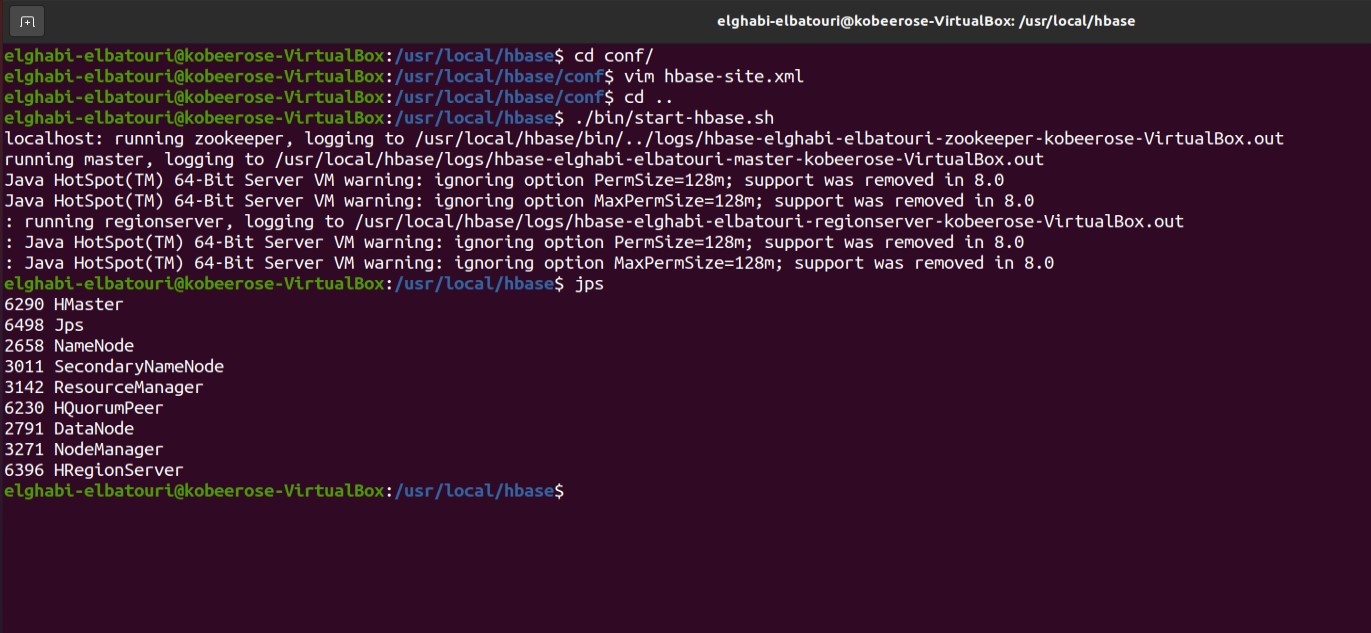
\includegraphics[width=1\linewidth]{Pictures/HBase/Configuring Hbase in Standalone & Pseudo-distributed mode/Configuring Hbase in Pseudo-distributed mode/Launching Hbase} 
\end{center} 
\caption{Launching Hbase} 
\end{figure}  \FloatBarrier
\\

\par Lorem ipsum dolor sit amet, consectetur adipiscing elit. Aliquam facilisis massa quis orci volutpat, ut dictum tellus pulvinar. Nam vulputate diam a leo dignissim varius. Aenean nec tellus malesuada, tristique libero vitae, lacinia nibh. Donec quam libero, accumsan sollicitudin massa a, dictum gravida mauris
\\
\begin{figure}[!htb] 
\begin{center} 
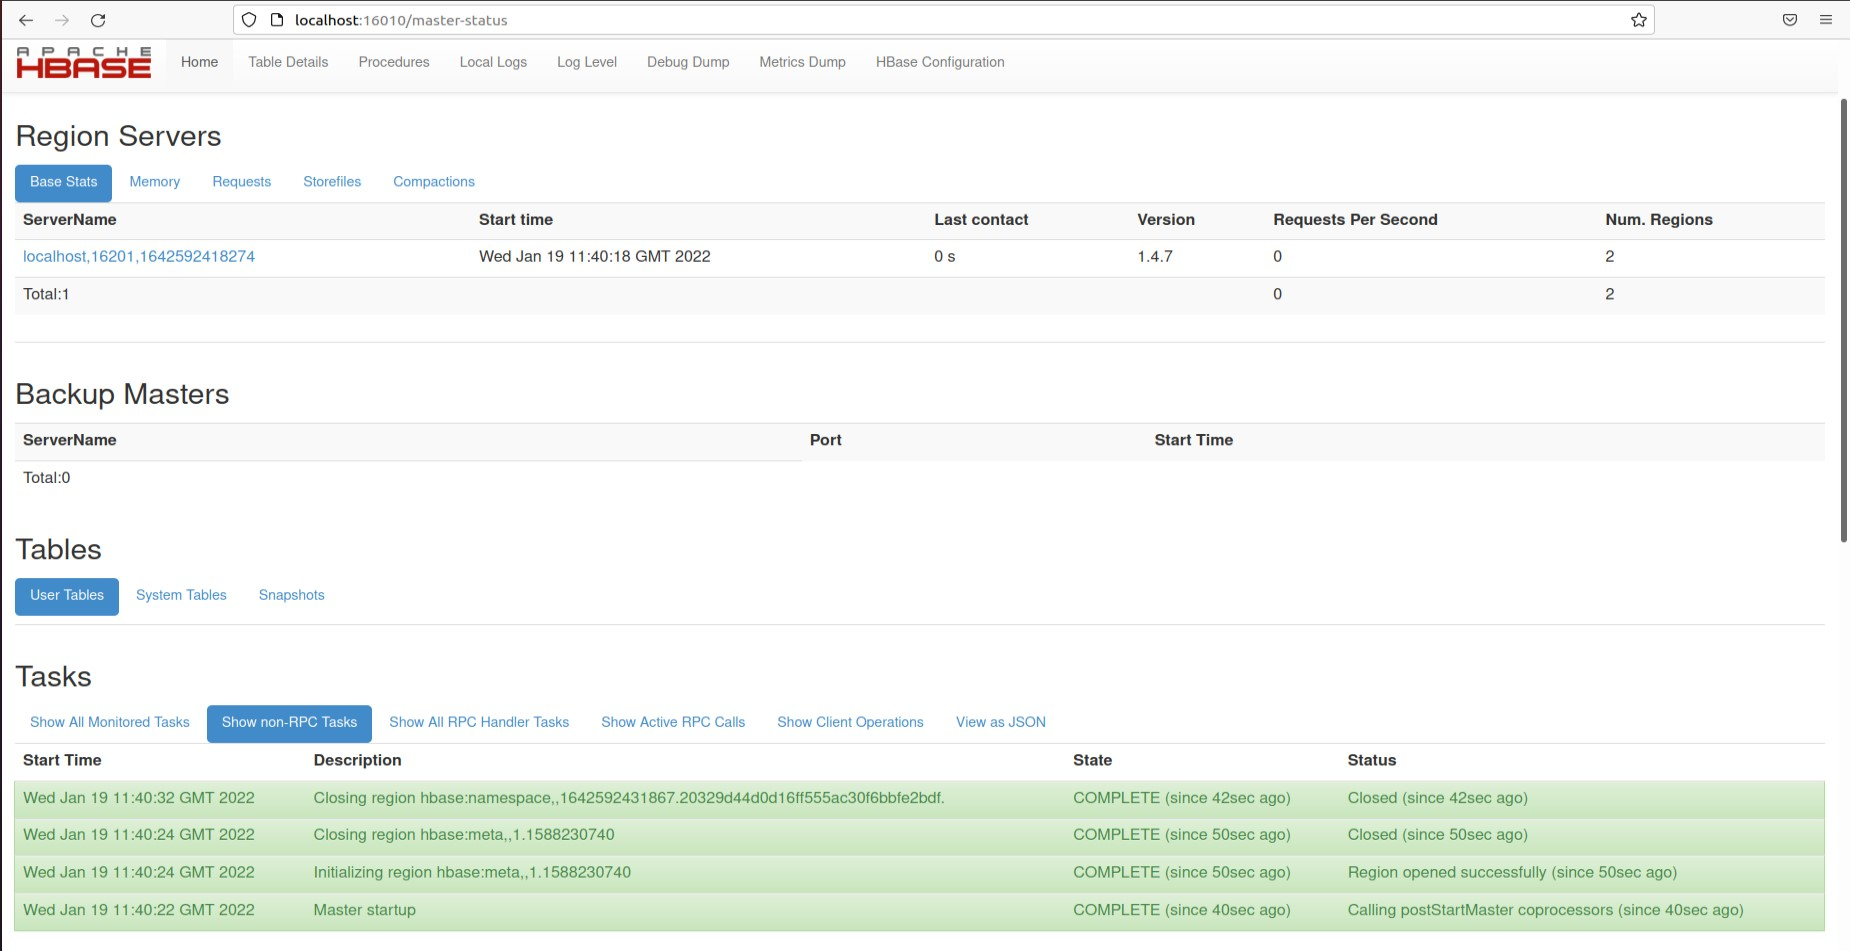
\includegraphics[width=1\linewidth]{Pictures/HBase/Configuring Hbase in Standalone & Pseudo-distributed mode/Configuring Hbase in Pseudo-distributed mode/Testing in browser} 
\end{center} 
\caption{Testing in browser} 
\end{figure}  \FloatBarrier
\\

\par Lorem ipsum dolor sit amet, consectetur adipiscing elit. Aliquam facilisis massa quis orci volutpat, ut dictum tellus pulvinar. Nam vulputate diam a leo dignissim varius. Aenean nec tellus malesuada, tristique libero vitae, lacinia nibh. Donec quam libero, accumsan sollicitudin massa a, dictum gravida mauris
\\
\begin{figure}[!htb] 
\begin{center} 
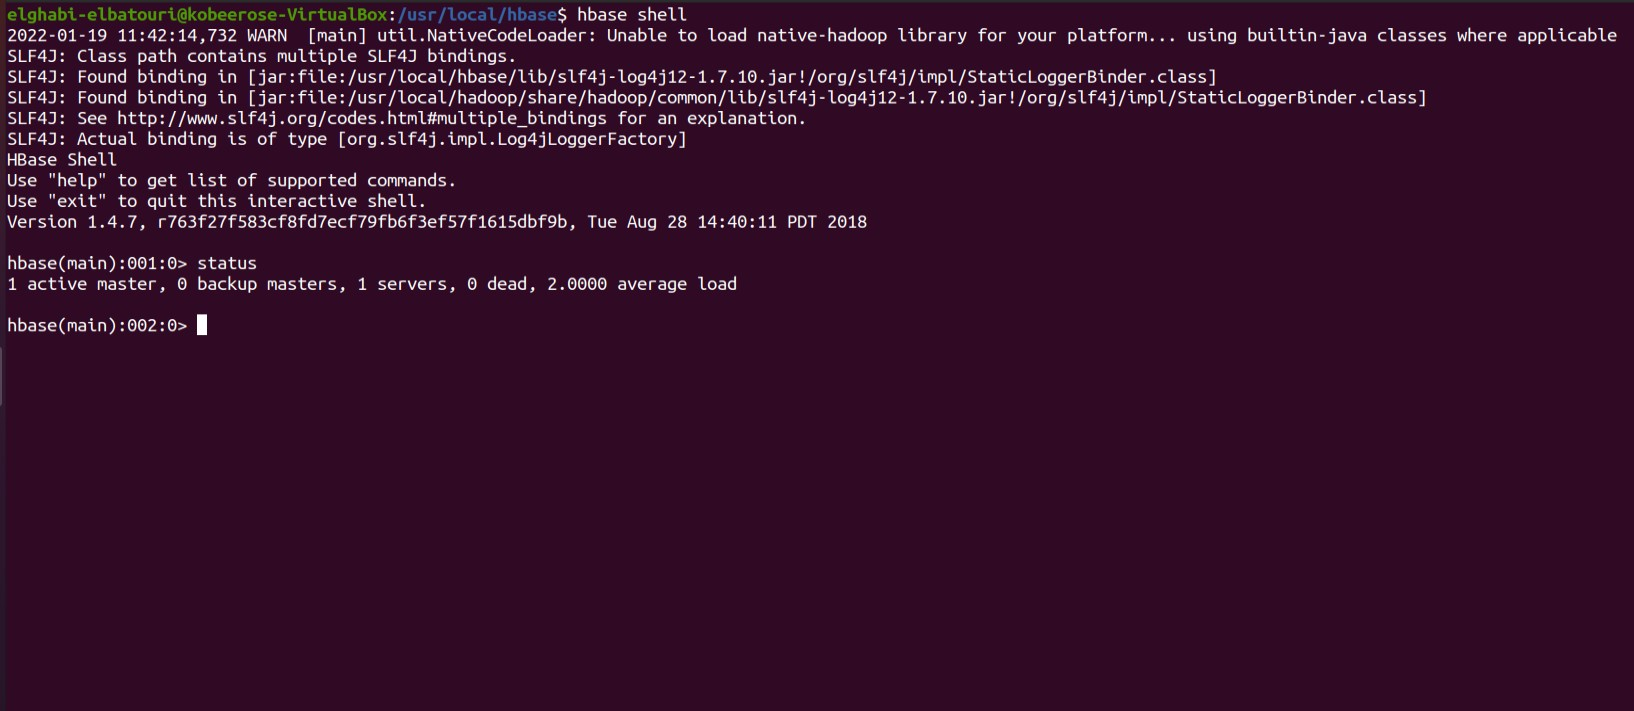
\includegraphics[width=1\linewidth]{Pictures/HBase/Configuring Hbase in Standalone & Pseudo-distributed mode/Configuring Hbase in Pseudo-distributed mode/Testing in Terminal} 
\end{center} 
\caption{Testing in Terminal} 
\end{figure}  \FloatBarrier
\\

\par Lorem ipsum dolor sit amet, consectetur adipiscing elit. Aliquam facilisis massa quis orci volutpat, ut dictum tellus pulvinar. Nam vulputate diam a leo dignissim varius. Aenean nec tellus malesuada, tristique libero vitae, lacinia nibh. Donec quam libero, accumsan sollicitudin massa a, dictum gravida mauris
\\
\begin{figure}[!htb] 
\begin{center} 
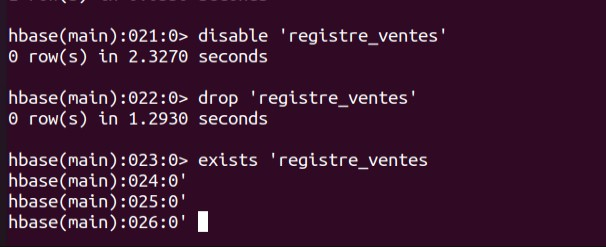
\includegraphics[width=1\linewidth]{Pictures/HBase/Configuring Hbase in Standalone & Pseudo-distributed mode/Configuring Hbase in Pseudo-distributed mode/Droping a table} 
\end{center} 
\caption{Droping a table} 
\end{figure}  \FloatBarrier
\\

\end{spacing}